\subsubsubsection{curve-double}

\begin{enumerate}
    \item \verb|Target|: Implement the addition of two same curve points. this is an incomplete addition, you can refer to The halo2 Book\cite{website:halo2-book} to learn more about it.
    \item \verb|Constraints logic|: See \ref{fig:curve-double-layout}.
    \item \verb|Constraints info and costs|:
    \begin{itemize}
        \item gadget-sub-nonnative num: 3
        \item gadget-add-nonnative num: 5
        \item gadget-mul-nonnative num: 4
        \item gadget-inv-nonnative num: 1
        \item gate type num: 14
            \begin{itemize}
                \item 8: U32AddManyGate\{2,3,5,7,9,11,13,15\}
                \item 1: ComparisonGate
                \item 1: ArithmeticGate
                \item 1: U32ArithmeticGate
                \item 1: U32SubtractionGate
                \item 2: U32RangeCheckGate\{0,8\}
            \end{itemize}
    \end{itemize}
\end{enumerate}

\begin{figure}[!ht]
    \centering
    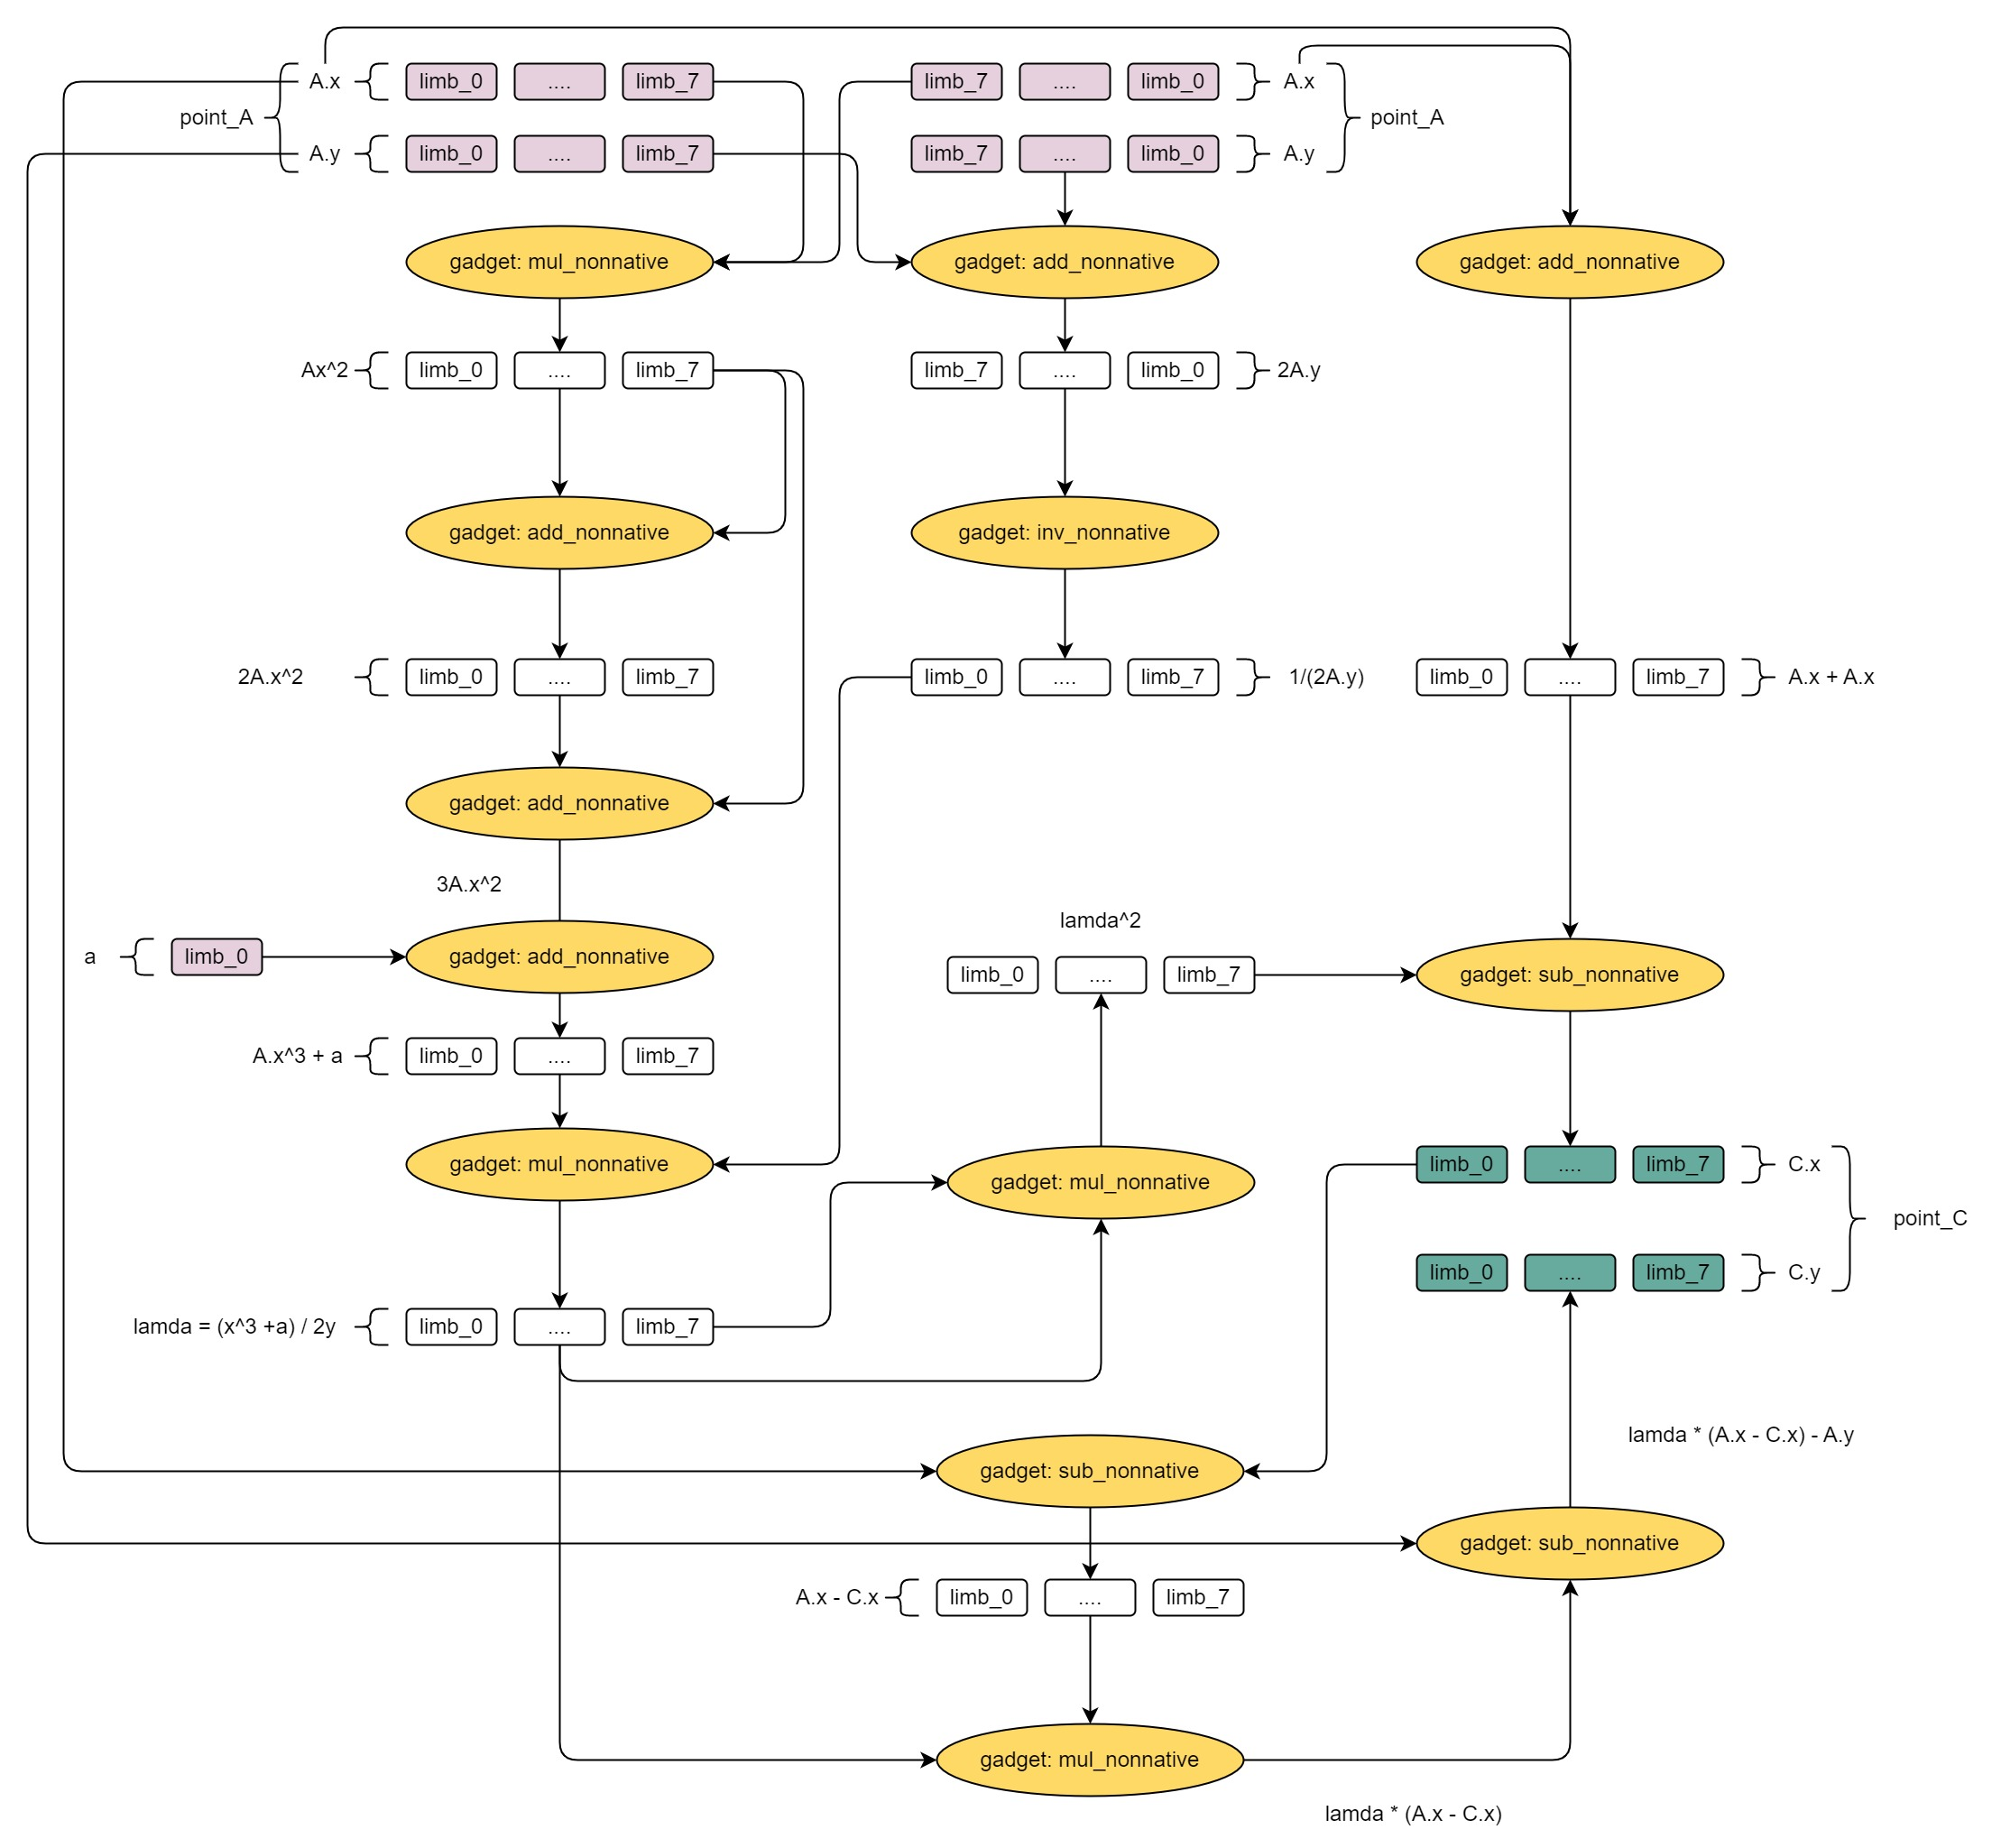
\includegraphics[width=0.6\textwidth]{curve-double-layout.jpg}
    \caption{curve-double layout}
    \label{fig:curve-double-layout}
\end{figure}
